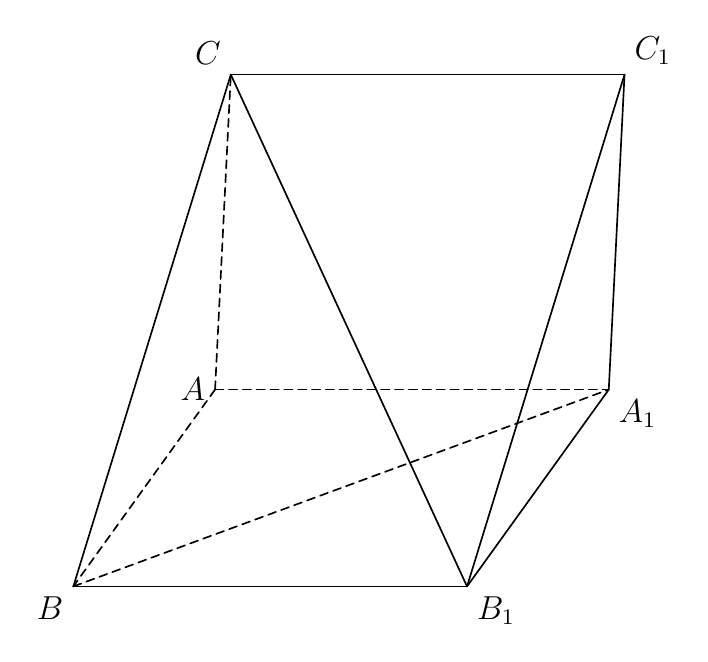
\begin{tikzpicture}[line width=.6pt,line join=round,line cap=round]
\coordinate (A) at (2.0,3.0);
\coordinate (C) at (2.2,7.0);
\coordinate (B) at (0.2,0.5);
\coordinate (A1) at (7.0,3.0);
\coordinate (C1) at (7.2,7.0);
\coordinate (B1) at (5.2,0.5);
% hidden edges
\draw[densely dashed] (A) -- (C);
\draw[densely dashed] (A) -- (B);
\draw[densely dashed] (A) -- (A1);
% solid prism edges
\draw (B) -- (C);
\draw (B) -- (B1);
\draw (C) -- (C1);
\draw (C1) -- (A1);
\draw (A1) -- (B1);
\draw (B1) -- (C1);
% auxiliary diagonals named in proof
\draw (C) -- (B1);
\draw[densely dashed] (B) -- (A1);
% labels
\node[left,font=\large] at (A) {$A$};
\node[above left,font=\large] at (C) {$C$};
\node[below left,font=\large] at (B) {$B$};
\node[below right,font=\large] at (A1) {$A_{1}$};
\node[above right,font=\large] at (C1) {$C_{1}$};
\node[below right,font=\large] at (B1) {$B_{1}$};
\end{tikzpicture}
